% !TEX root = ../main.tex
\section{实验\chinese{section}}
\subsection{实验题目}
WDT\_A实验
\subsection{实验目的}
WDT作为间隔定时器,定时间隔0.064ms,ISR内翻转P4.1状态。
\subsection{实验仪器和设备}
计算机、开发板、示波器、信号源、电源、Code Composer Studio v5、串口调试助手等。
\subsection{实验步骤}
\begin{lstlisting}[language=C]
/****************************************
--|RST P4.1|-->LED_Yellow
****************************************/
\end{lstlisting}
\par\indent 
使用看门狗定时器的间隔定时器模式,设置P4.0为输出,使用外部32768Hz晶振作为ACLK,采用中断模式。在中断服务程序中令P4.0口翻转,实现LED灯闪烁。
\subsection{程序清单}
\lstinputlisting{src/code/WDT.c}
\subsection{实验结果记录与分析}
\begin{figure}[htbp]
	\centering
	\caption{WDT}
	\label{WDT}
	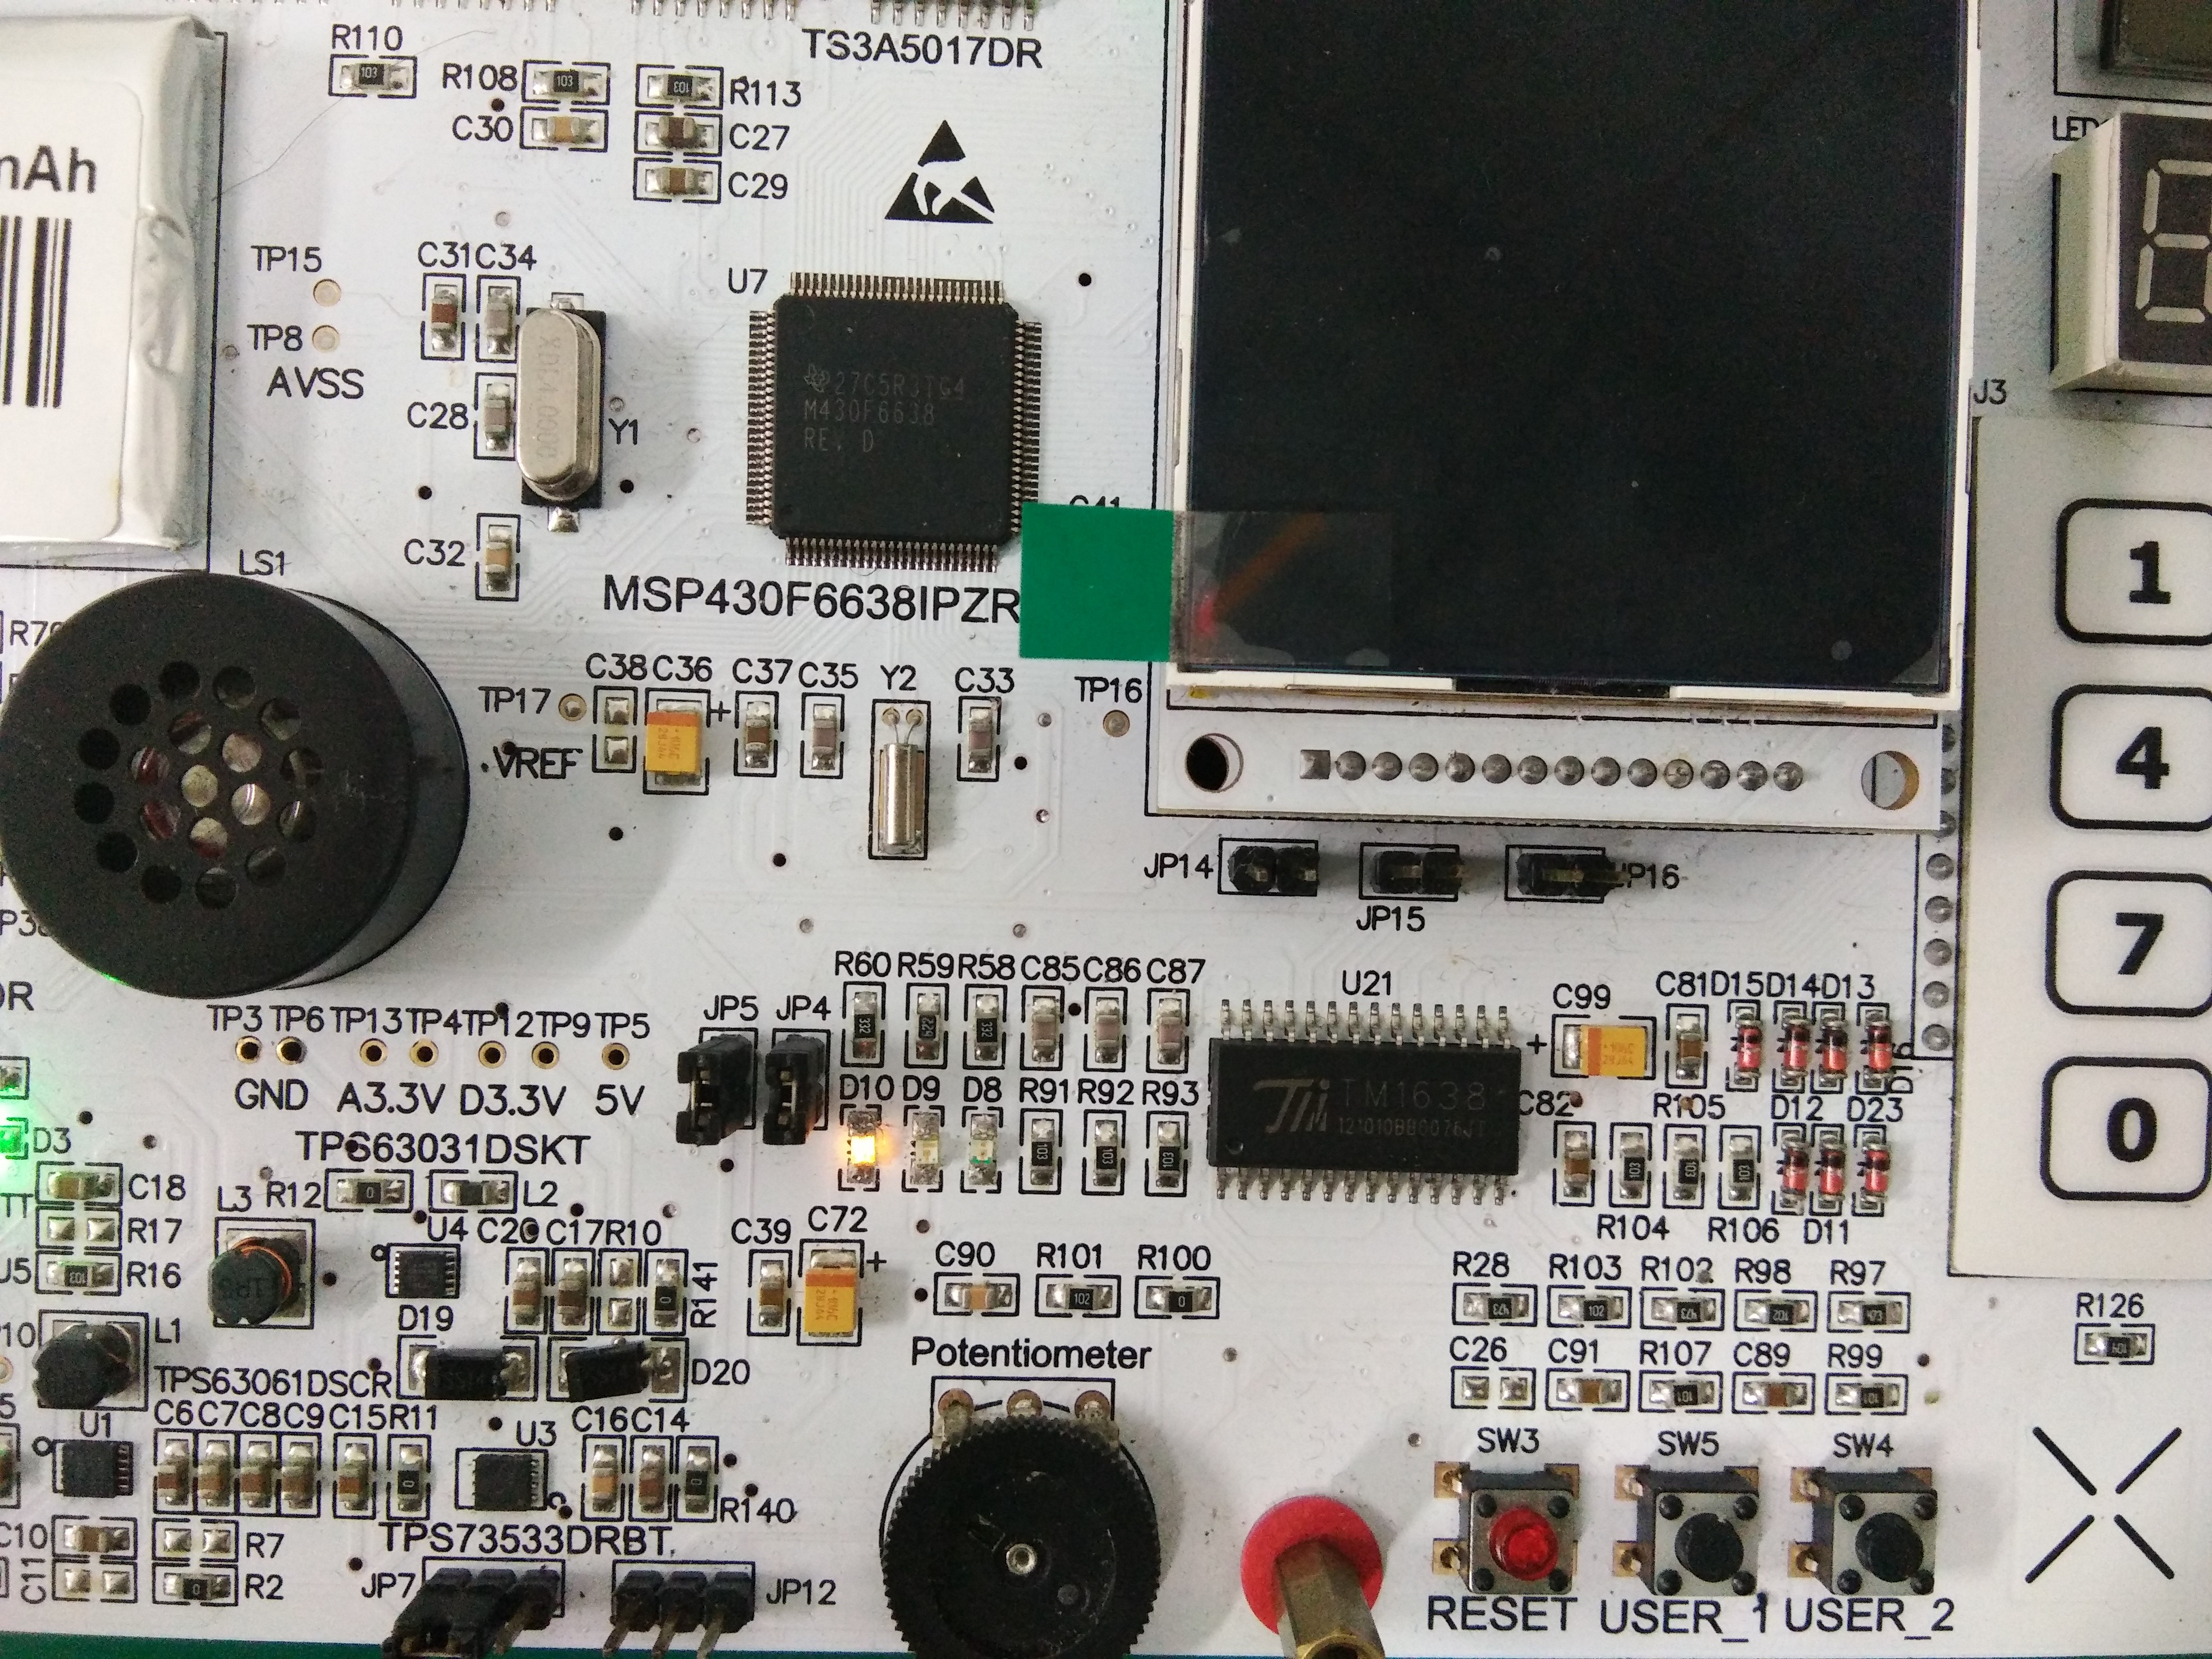
\includegraphics[width=8cm]{bitmap/jpg/WDT.jpg}
\end{figure}
\subsection{遇到的问题与解决方法}
\begin{enumerate}
	\item 在判断LED灯的闪烁上,一开始因为闪烁频率太高人眼无法察觉而误以为程序有错。算是增长了开发经验了。
\end{enumerate}

